\documentclass[answers]{exam}
\usepackage{longtable}
\usepackage{amsmath}
\usepackage{amssymb}
\usepackage{tikz}

% Bibliographic elements
\title{MATH3909 Chapter Four Notes}
\date{\today}
\author{Bow Valley College\\Data Management and Analytics}

% Formatting
\pagestyle{headandfoot}
\firstpageheader{MATH3909}{Chapter Four Notes}{\today}
\firstpageheadrule
\runningheader{MATH3909}{Chapter Four Notes}{\today}
\runningheadrule
\footer{}{\thepage}{}
\unframedsolutions

\begin{document}
    \begin{questions}
        \titledquestion{Prosecutor's Fallacy}\textbf{\thequestiontitle}

        Bow Valley College has purposed to implement random COVID screening of students
        using a rapid test. Currently 1 in 1000 Albertans have COVID. Using the Confusion
        Matrix for the rapid test, what is the probability a student has COVID given a
        positive test.
        \begin{longtable}{lp{3cm}p{3cm}}
            & \multicolumn{2}{c}{Actual COVID Infection} \\
            Test Result & Absent & Present\\
            \hline
            \endhead\\
            Positive &
            $1/100$ \par False Positive &
            $2/3$ \par True Positive \par Sensitivity\\\\
            Negative &
            $99/100$ \par True Negative \par Specificity &
            $$\frac{1}{3}$$ \par False Negative
        \end{longtable}
        \begin{solution}
            We apply Bayes' Theorem to find the probability of having COVID given a positive
            test.
            \begin{align*}
                \operatorname{\mathbb{P}}\left[ \text{Present} \middle\| \text{Positive} \right]
                & = 
                \operatorname{\mathbb{P}}\left[ \text{Positive} \middle\| \text{Present} \right]
                \cdot
                \frac{\operatorname{\mathbb{P}}\left[ \text{Present} \right]}
                {\operatorname{\mathbb{P}}\left[ \text{Positive} \right]}
                \\ & =
                \frac{\operatorname{\mathbb{P}}\left[ \text{Positive} \middle\| \text{Present} \right] \cdot \operatorname{\mathbb{P}}\left[ \text{Present} \right]}
                {\operatorname{\mathbb{P}}\left[ \text{Positive} \middle\| \text{Present} \right] \cdot \operatorname{\mathbb{P}}\left[ \text{Present} \right] + \operatorname{\mathbb{P}}\left[ \text{Positive} \middle\| \text{Absent} \right] \cdot \operatorname{\mathbb{P}}\left[ \text{Absent} \right]}
                \\ & =
                \frac{1}{1 + \frac{\operatorname{\mathbb{P}}\left[ \text{Positive} \middle\| \text{Absent} \right] \cdot \operatorname{\mathbb{P}}\left[ \text{Absent} \right]}{\operatorname{\mathbb{P}}\left[ \text{Positive} \middle\| \text{Present} \right] \cdot \operatorname{\mathbb{P}}\left[ \text{Present} \right]}}
                \\ & =
                \frac{1}{1 + \frac{\frac{1}{100} \cdot \frac{999}{1000}}{\frac{2}{3} \cdot \frac{1}{1000}}}
                \\ & =
                \frac{1}{1 + \frac{2997}{200}}
                \\ & =
                \frac{200}{3197}
            \end{align*}
            Thus there is only a ${\approx}6.3\%$ chance the randomly selected student who
            tested positive actually has COVID.
        \end{solution}
        \titledquestion{Monty Hall Problem}\textbf{\thequestiontitle}

        The Monty Hall Problem is a game of chance with conditional information:
        \begin{enumerate}
            \item The game begins with a prize randomly hidden behind one of three doors.
            \item The contestant chooses an initial door out of the three.
            \item A door that neither the contestant has chosen, nor containing a prize is
            then opened.
            \item The contestant can then optionally choose to switch their choice of doors
            to the remaining unopened door.
            \item Finally the prize door is revealed. If it is the final choice of the
            contestant then the contestant wins, otherwise they lose.
        \end{enumerate}
        The counterintuitive result of this game is that the optimum strategy is for the
        contestant to always switch their choice of doors, as that has a two thirds chance
        of winning.
        \begin{solution}
            We will use a tree diagram to calculate the theoretical probability of winning
            conditioned on the strategy of switching the choice of doors.

            Tree diagrams allow for the calculation of discrete, or enumerable,
            probabilities by observing that the joint probability of any finite sequence of
            events $E_1, \dots, E_n$ can be recursively factored into a sequence of
            conditional probabilities. We will start by writing the events in reverse order:
            \begin{align*}
                \operatorname{\mathbb{P}}\left[ E_n, \dots, E_1 \right]
                & =
                \operatorname{\mathbb{P}}\left[ E_n \middle\| E_{n-1} \dots, E_1 \right]
                \cdot
                \operatorname{\mathbb{P}}\left[ E_{n-1}, \dots, E_1 \right]
                \\ & =
                \operatorname{\mathbb{P}}\left[ E_n \middle\| E_{n-1} \dots, E_1 \right]
                \cdot
                \operatorname{\mathbb{P}}\left[ E_{n-1} \middle\| E_{n-2} \dots, E_1 \right]
                \cdot
                \operatorname{\mathbb{P}}\left[ E_{n-2}, \dots, E_1 \right]
                \\ & \; \; \vdots
                \\ & =
                \operatorname{\mathbb{P}}\left[ E_n \middle\| E_{n-1} \dots, E_1 \right]
                \cdot
                \operatorname{\mathbb{P}}\left[ E_{n-1} \middle\| E_{n-2} \dots, E_1 \right]
                \cdot
                \\ & \qquad \vdots
                \\ & \qquad \cdot
                \operatorname{\mathbb{P}}\left[ E_2 \middle\| E_1 \right]
                \cdot
                \operatorname{\mathbb{P}}\left[ E_1 \right]
            \end{align*}
            Each conditional probability is the probability of visiting the next branch
            given the current branch. In many circumstances the probability of the next
            event conditioned on the current event is much more easily modelled than the
            overall joint probability. In this example we will write our tree starting from
            the left. At each node of the tree we write the outcome and the conditional
            probability of the outcome.
            
            For the Monty Hall Problem their are two important observations: first, the
            conditional probabilities of the branches within the preceding branch are
            uniform; second, the contestants choice of door is independent of the assignment
            of the prize. The last observation simply asserts that the contestant does not
            possess psychic abilities. The outcomes of each branch is simply one of the
            three possible doors. To calculate the probability of winning conditioned on
            switching we sum all the joint probabilities of winning and using the switching
            strategy and divide by all the joint probabilities of either winning or losing
            under the switching strategy. The denominator is the marginal probability of the
            switching strategy.
            \begin{align*}
                \operatorname{\mathbb{P}}\left[ \text{Win} \middle\| \text{Switch} \right]
                & =
                \frac{\operatorname{\mathbb{P}}\left[ \text{Win},  \text{Switch} \right]}
                {\operatorname{\mathbb{P}}\left[ \text{Win},  \text{Switch} \right] + \operatorname{\mathbb{P}}\left[ \text{Lose},  \text{Switch} \right]}
                \\ & =
                \frac{6 \cdot \frac{1}{3} \cdot \frac{1}{3}}
                {6 \cdot \frac{1}{3} \cdot \frac{1}{3} + 6 \cdot \frac{1}{3} \cdot \frac{1}{3} \frac{1}{2}}
                \\ & =
                \frac{2}{3}
            \end{align*}
            \begin{center}
                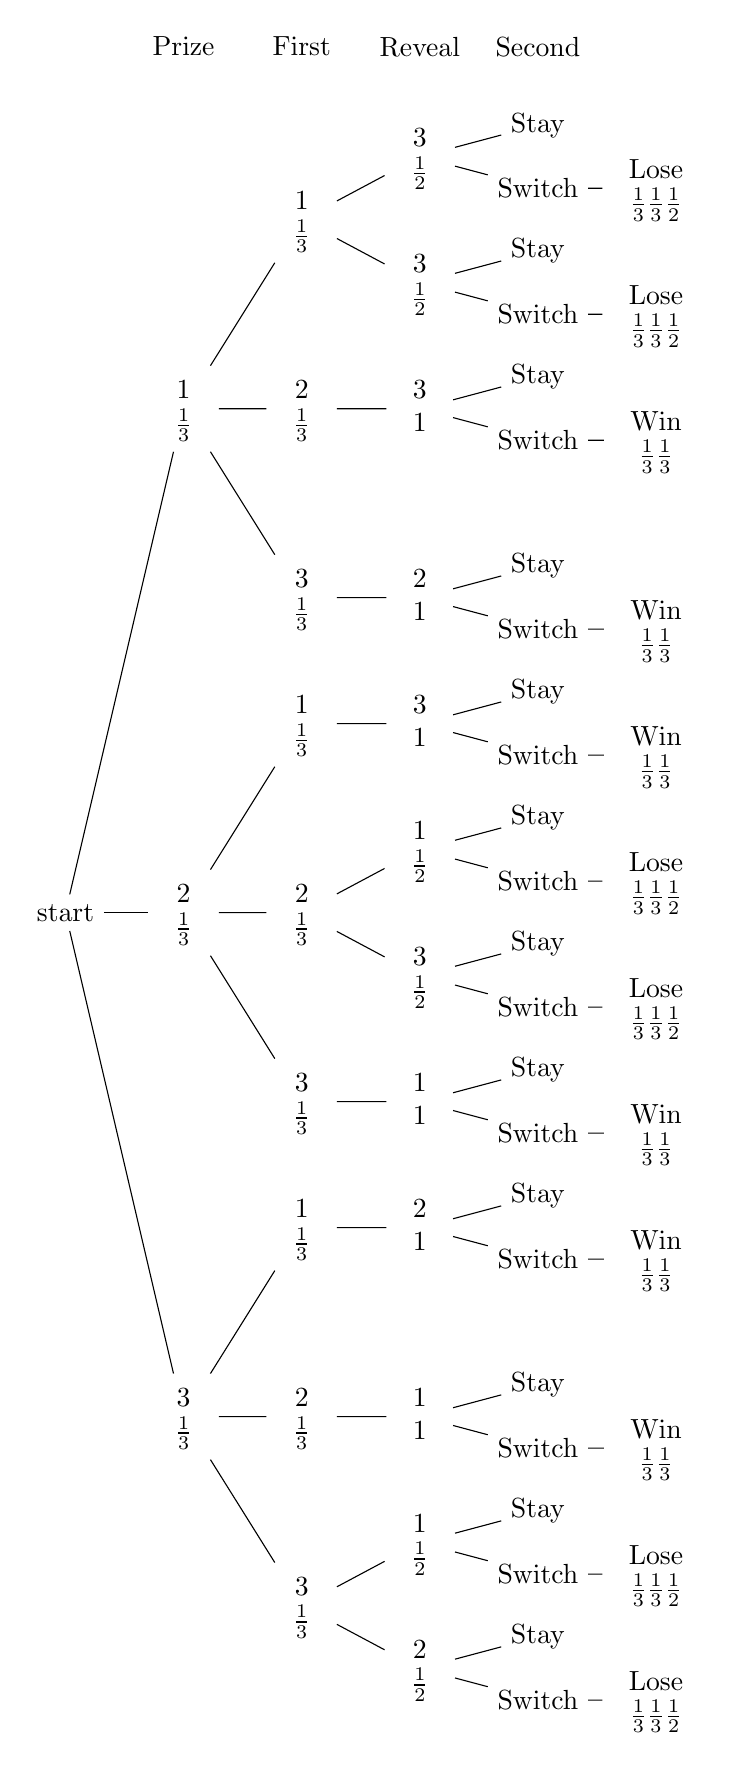
\begin{tikzpicture}
                    \node {} [grow = right]
                        child { node {Prize} edge from parent [draw = none]
                            child { node {First}  edge from parent [draw = none]
                                child { node {Reveal}  edge from parent [draw = none]
                                    child { node {Second}  edge from parent [draw = none] }
                                }
                            }
                        };
                    \node at (0, -11) {start} [grow = right, sibling distance = 64mm]
                        child { node {\begin{tabular}{c} 3 \\ $\frac{1}{3}$ \end{tabular}} [sibling distance = 24mm]
                            child { node {\begin{tabular}{c} 3 \\ $\frac{1}{3}$ \end{tabular}} [sibling distance = 16mm]
                                child { node {\begin{tabular}{c} 2 \\ $\frac{1}{2}$ \end{tabular}} [sibling distance = 8mm]
                                    child { node {Switch}
                                        child { node {\begin{tabular}{c} Lose \\ $\frac{1}{3}\frac{1}{3}\frac{1}{2}$ \end{tabular}} }
                                    }
                                    child { node {Stay} }
                                }
                                child { node {\begin{tabular}{c} 1 \\ $\frac{1}{2}$ \end{tabular}} [sibling distance = 8mm]
                                    child { node {Switch}
                                        child { node {\begin{tabular}{c} Lose \\ $\frac{1}{3}\frac{1}{3}\frac{1}{2}$ \end{tabular}} }
                                    }
                                    child { node {Stay} }
                                }
                            }
                            child { node {\begin{tabular}{c} 2 \\ $\frac{1}{3}$ \end{tabular}}
                                child { node {\begin{tabular}{c} 1 \\ 1 \end{tabular}} [sibling distance = 8mm]
                                    child { node {Switch}
                                        child { node {\begin{tabular}{c} Win \\ $\frac{1}{3}\frac{1}{3}$ \end{tabular}} }
                                    }
                                    child { node {Stay} }
                                }
                            }
                            child { node {\begin{tabular}{c} 1 \\ $\frac{1}{3}$ \end{tabular}}
                                child { node {\begin{tabular}{c} 2 \\ 1 \end{tabular}} [sibling distance = 8mm]
                                    child { node {Switch}
                                        child { node {\begin{tabular}{c} Win \\ $\frac{1}{3}\frac{1}{3}$ \end{tabular}} }
                                    }
                                    child { node {Stay} }
                                }
                            }
                        }
                        child { node {\begin{tabular}{c} 2 \\ $\frac{1}{3}$ \end{tabular}} [sibling distance = 24mm]
                            child { node {\begin{tabular}{c} 3 \\ $\frac{1}{3}$ \end{tabular}}
                                child { node {\begin{tabular}{c} 1 \\ 1 \end{tabular}} [sibling distance = 8mm]
                                    child { node {Switch}
                                        child { node {\begin{tabular}{c} Win \\ $\frac{1}{3}\frac{1}{3}$ \end{tabular}} }
                                    }
                                    child { node {Stay} }
                                }
                            }
                            child { node {\begin{tabular}{c} 2 \\ $\frac{1}{3}$ \end{tabular}} [sibling distance = 16mm]
                                child { node {\begin{tabular}{c} 3 \\ $\frac{1}{2}$ \end{tabular}} [sibling distance = 8mm]
                                    child { node {Switch}
                                        child { node {\begin{tabular}{c} Lose \\ $\frac{1}{3}\frac{1}{3}\frac{1}{2}$ \end{tabular}} }
                                    }
                                    child { node {Stay} }
                                }
                                child { node {\begin{tabular}{c} 1 \\ $\frac{1}{2}$ \end{tabular}} [sibling distance = 8mm]
                                    child { node {Switch}
                                        child { node {\begin{tabular}{c} Lose \\ $\frac{1}{3}\frac{1}{3}\frac{1}{2}$ \end{tabular}} }
                                    }
                                    child { node {Stay} }
                                }
                            }
                            child { node {\begin{tabular}{c} 1 \\ $\frac{1}{3}$ \end{tabular}}
                                child { node {\begin{tabular}{c} 3 \\ 1 \end{tabular}} [sibling distance = 8mm]
                                    child { node {Switch}
                                        child { node {\begin{tabular}{c} Win \\ $\frac{1}{3}\frac{1}{3}$ \end{tabular}} }
                                    }
                                    child { node {Stay} }
                                }
                            }
                        }
                        child { node {\begin{tabular}{c} 1 \\ $\frac{1}{3}$ \end{tabular}} [sibling distance = 24mm]
                            child { node {\begin{tabular}{c} 3 \\ $\frac{1}{3}$ \end{tabular}}
                                child { node {\begin{tabular}{c} 2 \\ 1 \end{tabular}} [sibling distance = 8mm]
                                    child { node {Switch}
                                        child { node {\begin{tabular}{c} Win \\ $\frac{1}{3}\frac{1}{3}$ \end{tabular}} }
                                    }
                                    child { node {Stay} }
                                }
                            }
                            child { node {\begin{tabular}{c} 2 \\ $\frac{1}{3}$ \end{tabular}}
                                child { node {\begin{tabular}{c} 3 \\ 1 \end{tabular}} [sibling distance = 8mm]
                                    child { node {Switch}
                                        child { node {\begin{tabular}{c} Win \\ $\frac{1}{3}\frac{1}{3}$ \end{tabular}} }
                                    }
                                    child { node {Stay} }
                                }
                            }
                            child { node {\begin{tabular}{c} 1 \\ $\frac{1}{3}$ \end{tabular}} [sibling distance = 16mm]
                                child { node {\begin{tabular}{c} 3 \\ $\frac{1}{2}$ \end{tabular}} [sibling distance = 8mm]
                                    child { node {Switch}
                                        child { node {\begin{tabular}{c} Lose \\ $\frac{1}{3}\frac{1}{3}\frac{1}{2}$ \end{tabular}} }
                                    }
                                    child { node {Stay} }
                                }
                                child { node {\begin{tabular}{c} 3 \\ $\frac{1}{2}$ \end{tabular}} [sibling distance = 8mm]
                                    child { node {Switch}
                                        child { node {\begin{tabular}{c} Lose \\ $\frac{1}{3}\frac{1}{3}\frac{1}{2}$ \end{tabular}} }
                                    }
                                    child { node {Stay} }
                                }
                            }
                        };
                \end{tikzpicture}
            \end{center}
        \end{solution}
    \end{questions}
\end{document}